\documentclass[12pt, letterpaper]{article}

% --- PACKAGES ---
\usepackage[utf8]{inputenc}
\usepackage[T1]{fontenc}
\usepackage{mathpazo} % Palatino - perfect for algebraic geometry text
\usepackage[margin=1in]{geometry}
\usepackage{amsmath, amssymb, amsfonts, amsthm}
\usepackage{mathrsfs} % For sheaf notation \mathscr{O}
\usepackage{fancyhdr} 
\usepackage{xcolor}
\usepackage{tikz} 
\usetikzlibrary{shapes.geometric, arrows.meta}
\usepackage[most]{tcolorbox} 

% --- SUBJECT SPECIFIC MACROS ---
\newcommand{\CC}{\mathbb{C}} % Complex Plane
\newcommand{\RR}{\mathbb{R}} % Real Numbers
\newcommand{\ZZ}{\mathbb{Z}} % Integers
\newcommand{\PP}{\mathbb{P}} % Projective Space
\newcommand{\HH}{\mathbb{H}} % Upper Half Plane
\newcommand{\Lat}{\Lambda}   % Lattice
\newcommand{\Div}{\mathrm{Div}} % Divisors
\newcommand{\ord}{\mathrm{ord}} % Order
\newcommand{\sheaf}{\mathscr{O}} % Structure Sheaf

% --- COLORS & STYLE ---
\definecolor{themecolor}{RGB}{40, 60, 100} % Deep Navy (Academic/Formal)
\definecolor{gridcolor}{RGB}{220, 220, 220} 

% --- PAGE HEADER/FOOTER ---
\pagestyle{fancy}
\fancyhf{}
\fancyhead[L]{\small \textsc{Riemann Surfaces \& Algebraic Curves}}
\fancyhead[R]{\small \today}
\fancyfoot[C]{\thepage}
\renewcommand{\headrulewidth}{0.4pt}

% --- PROBLEM COMMAND ---
\newcounter{probcount}
\newcommand{\makequestion}[2]{
	\clearpage
	\stepcounter{probcount}
	
	% Problem Statement Box
	\begin{tcolorbox}[
		enhanced,
		colback=white,
		colframe=themecolor,
		coltitle=white,
		fonttitle=\bfseries\large,
		title={Exercise \theprobcount: #1},
		sharp corners=south,
		drop fuzzy shadow,
		boxrule=0.5mm,
		top=6mm, bottom=6mm
		]
		%\large 
		#2
	\end{tcolorbox}
	
	% Workspace
	\vfill
	\begin{center}
		\begin{tikzpicture}
			% A subtle dot grid for algebraic derivations
			\draw[step=0.5cm,gridcolor,very thin, dash pattern=on 0.5pt off 1.5pt] (0,0) grid (16,14);
		\end{tikzpicture}
	\end{center}
	\vfill
}

% --- TITLE PAGE SETUP ---
\title{
	\vspace{2cm}
	\begin{tcolorbox}[colback=themecolor, colframe=themecolor, sharp corners]
		\centering \color{white}
		\Huge \textbf{Elliptic Curves}\\
		\vspace{0.5em}
		\Large \textit{From Riemann Surfaces to Arithmetic Geometry}
	\end{tcolorbox}
}
\author{\textbf{Research Notebook}}
\date{\today}

% --- DOCUMENT START ---
\begin{document}
	
	% 1. COVER PAGE
	\begin{titlepage}
		\centering
		\maketitle
		\thispagestyle{empty}
		
		\vspace{2cm}
		
		% TikZ Visualization: A Torus (Genus 1 Surface) with cycles
		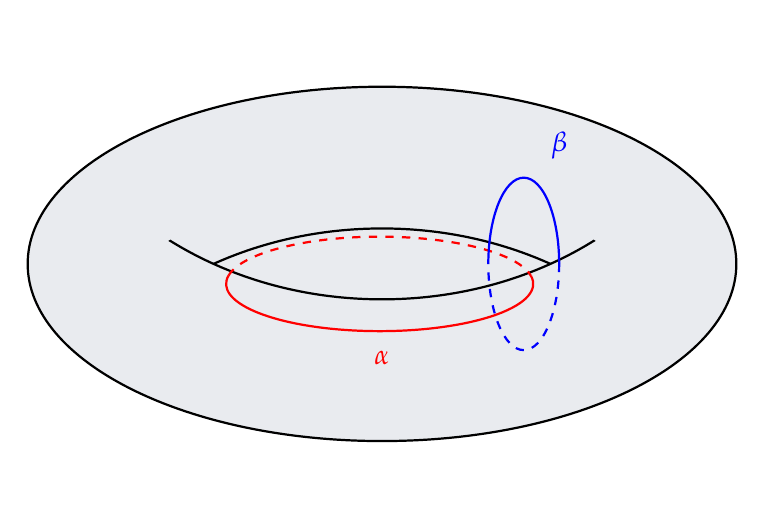
\begin{tikzpicture}[scale=1.5]
			\useasboundingbox (-3,-2) rectangle (3,2);
			
			% Torus Body
			\draw[thick, fill=themecolor!10] (0,0) ellipse (3cm and 1.5cm);
			
			% The Hole
			\begin{scope}
				\clip (0,-1.8) ellipse (3cm and 2.5cm);
				\draw[thick] (0,2.2) ellipse (3cm and 2.5cm);
			\end{scope}
			\begin{scope}
				\clip (0,2.2) ellipse (3cm and 2.5cm);
				\draw[thick] (0,-2.2) ellipse (3cm and 2.5cm);
			\end{scope}
			
			% Cycle Alpha (Horizontal)
			\draw[red, thick] (-1.3, -0.1) arc (170:370:1.3 and 0.4);
			\draw[red, dashed, thick] (-1.3, -0.1) arc (170:10:1.3 and 0.4);
			\node[red] at (0, -0.8) {$\alpha$};
			
			% Cycle Beta (Vertical wrap)
			\draw[blue, thick] (1.5, 0) arc (0:180:0.3 and 0.73); 
			\draw[blue, dashed, thick] (1.5, 0) arc (0:-180:0.3 and 0.73);
			\node[blue] at (1.5, 1) {$\beta$};
			
			\node at (0,-2.5) {\small $E(\CC) \cong \CC / \Lat$};
		\end{tikzpicture}
		
		\vfill
		\begin{center}
			\large \textbf{Subject:} Complex Analysis \& Algebraic Geometry
		\end{center}
	\end{titlepage}
	
	% 2. PROBLEMS
	
	\makequestion{The Weierstrass $\wp$-function}{
		Let $\Lat = \ZZ\omega_1 + \ZZ\omega_2$ be a lattice in $\CC$. The Weierstrass $\wp$-function is defined as:
		$$ \wp(z; \Lat) = \frac{1}{z^2} + \sum_{\omega \in \Lat \setminus \{0\}} \left( \frac{1}{(z-\omega)^2} - \frac{1}{\omega^2} \right) $$
		Prove that $\wp(z)$ is an elliptic function with periods $\Lat$ and show that it satisfies the differential equation:
		$$ (\wp'(z))^2 = 4\wp(z)^3 - g_2 \wp(z) - g_3 $$
		where $g_2 = 60 \sum_{\omega \neq 0} \omega^{-4}$ and $g_3 = 140 \sum_{\omega \neq 0} \omega^{-6}$.
	}
	
	\makequestion{Projective Closure in $\PP^2$}{
		Consider the affine curve $C_0$ defined by $y^2 = x^3 + ax + b$ over a field $K$.
		\begin{enumerate}
			\item Homogenize the equation to find the projective closure $C$ in $\PP^2$ with coordinates $[X:Y:Z]$.
			\item Determine the points at infinity (where $Z=0$).
			\item Prove that the point at infinity is a non-singular point of the curve.
		\end{enumerate}
	}
	
	\makequestion{Divisors and Riemann-Roch}{
		Let $X$ be a compact Riemann surface of genus $g$. For a divisor $D \in \Div(X)$, denote $l(D) = \dim_\CC H^0(X, \sheaf(D))$.
		
		State the **Riemann-Roch Theorem** relating $l(D)$, $l(K-D)$, and $\deg(D)$. 
		
		Then, apply it to the case where $X$ is an elliptic curve ($g=1$) and $D = P$ (a single point) to find the dimension of the space of meromorphic functions with at most a simple pole at $P$.
	}
	
\end{document}